\documentclass[final, notable, nolof, nolot, 11pt, nocover]{fithesis3}

%% The following section sets up the other used packages.
\usepackage[main=english]{babel}
\usepackage{graphicx}
\usepackage{algorithm}
\usepackage{algpseudocode}
\usepackage{algorithmicx}
\usepackage{amsmath}
\usepackage{mathptmx}
\usepackage{stfloats}
\usepackage{textcase}
\usepackage{esvect}
\usepackage{epstopdf}
\usepackage{wrapfig}
\usepackage{pdfpages}
\usepackage{subfigure}
\usepackage{makeidx}
\usepackage[textsize=small,colorinlistoftodos,disable]{todonotes}
\usepackage{textcomp}
\usepackage{chngcntr}


%\usepackage{verbatim}
%\usepackage{showframe}

%% The following section sets up the metadata of the thesis.
\thesissetup{
    university    = mu,
    faculty       = fi,
    type          = r,
    author        = Katarína Furmanová,
    gender        = m,
    advisor       = {prof. Jiří Sochor \\ \textbf{Co-Advisor:} assoc. prof. Barbora Kozlíková},
    title         = {Visualization and Visual Analysis of Intermolecular Interactions of Proteins},
    TeXtitle      = {Visualization and Visual Analysis of Intermolecular Interactions of Proteins},
    keywords      = {protein, protein-protein interactions, visualization, cavity, protein void, tunnel, trajectory, contact zone},
    TeXkeywords   = {protein, protein-protein interactions, visualization, cavity, protein void, tunnel, contact zone, CAVER Analyst},
}


\thesislong{abstract}{

}

\thesislong{thanks}{

}

%% The following section sets up the bibliography.
\usepackage{csquotes}
%\usepackage[             
%  backend=biber,         
%  bibstyle=numeric,          
%  citestyle=numeric-comp, 
%  sorting=none,           
%  sortlocale=auto,
%  maxnames=3,
%  firstinits=true         
%]{biblatex}  


%\renewbibmacro*{journal}{%
%  \iffieldundef{journaltitle}
%    {}
%    {\printtext[journaltitle]{%
%       \printfield[noformat]{journaltitle}%
%       \setunit{\subtitlepunct}%
%       \printfield[noformat]{journalsubtitle}}}}
       
%\renewbibmacro*{booktitle}{%
%  \iffieldundef{booktitle}
%    {}
%    {\printtext[booktitle]{%
%       \printfield[noformat]{booktitle}%
%       \setunit{\subtitlepunct}%
%       \printfield[noformat]{booksubtitle}}}}
%       
       
%\DeclareFieldFormat{titlecase}{\MakeSentenceCase{#1}}     
%\renewcommand*{\bibfont}{\small}
%\addbibresource{thesis.bib}

% Defines usefull commands.
\newcommand{\ie}{i.e.,~}
\newcommand{\eg}{e.g.,~}

% The following configures the algorithm package.
\renewcommand{\algorithmicrequire}{\textbf{Input:}}
\renewcommand{\algorithmicensure}{\textbf{Output:}}

\newcommand{\var}[1]{\textit{#1}}

% The following configures the subfigure.
\renewcommand{\thesubfigure}{(\Alph{subfigure})}

% The following section sets up the index.
\makeindex

\pdfminorversion=4

%\emergencystretch=1em

\begin{document}

%Makes the \part command work.
\pdfstringdefDisableCommands{%
	\let\MakeUppercase\relax
}

\listoftodos

%%%%%%%%%%%%%%%%%%%%%%%%%%%%%%%%%%%%%%%%%%%
%%%%%%%%%%%%%%%%%%%%%%%%%%%%%%%%%%%%%%%%%%%
%%%%%%%%%%%%%%%%%%%%%%%%%%%%%%%%%%%%%%%%%%%
%%%%%%%%%%%%%%%%%%%%%%%%%%%%%%%%%%%%%%%%%%%
%%%%%%%%%%%%%%%%%%%%%%%%%%%%%%%%%%%%%%%%%%%
\label{Sec:Overview}

%%%%%%%%%%%%%%%%%%%%%%%%%%%%%%%%%%%%%%%%%%%
%%%%%%%%%%%%%%%%%%%%%%%%%%%%%%%%%%%%%%%%%%%
%%%%%%%%%%%%%%%%%%%%%%%%%%%%%%%%%%%%%%%%%%%
\chapter{Introduction}
\label{Sec:Intro}
Proteins are highly complex macromolecules that are vital to biochemical processes taking place in each living organism. Weather alone or as a part of multi-unit complexes, they facilitate vast field of functions such as catalysing chemical reactions, transporting molecules across the cells or replication of DNA. In these processes the ability of a protein to interact with other molecules plays a defining role. 

Since the proper understanding of protein interactions contributes to advances in medicine, pharmaceutics or even agriculture, the study of interaction patterns of proteins has been at the forefront of biochemical research for decades. Unfortunately, the complexity of protein structures and the necessity for expensive and time consuming in-vitro experiments make the progress in the area slow. Many computational tools aim to support this research by simulating the experiments in-silico and thus reducing the costs. However, these tools can produce a vast amounts of data. For example molecular dynamics simulations can mimic the movement of millions of atoms over a given period of time. It is virtually impossible to identify significant patterns by simply observing such simulation. Another example are the protein-protein docking simulations that predict the possible ways two or more proteins interact together. Here the output often comprises of tens to hundreds of possible conformations that the domain expert needs to analyse individually one by one.

Therefore, visualization and visual analysis tools became inherent part of proteomic research both as guidance during the experiments as well as for validation and analysis of results by the domain experts.  The main aim of these tools is to speed up the analysis process by - often interactively - extracting the important features of the data and conveying them in such way, that previously hardly observable patterns and relationships become more prominent. Although much has been done in the field of molecular visualization in the past decades, there are still areas and problems that are not currently addressed. 

%Particularly the area of protein-protein interactions remains largely untouched by scientific literature in terms of visual analysis. 

\section{Biochemical Definitions}
\label{Sec:Chem}
Although this thesis deals with the research in the field of visualization and visual analysis, it also ventures into the field of biochemistry. It is therefore inevitable to clarify the basic biochemical terms that will occur throughout the thesis and are important for its proper understanding. This section shall provide the reader with all the necessary knowledge.

\subsection{Protein Structures}
\label{Sec:structures}
Proteins are complex molecules formed by one or more chains of amino acids. Amino acids are basic building blocks of all living organisms. There are approximately 500 known amino acids, but only 20 standard amino acids are encoded in genetic code. Each of them consists of \textit{carboxyl group} ($-COOH$), an \textit{amino group} ($-NH_2$) and a unique \textit{side chain} ($-R$) that defines its properties. The three groups are connected by a carbon atom, also called an \textit{alpha carbon} $C_\alpha$. See figure \ref{Fig:aa} a).

\begin{figure}[H]
  \centering
  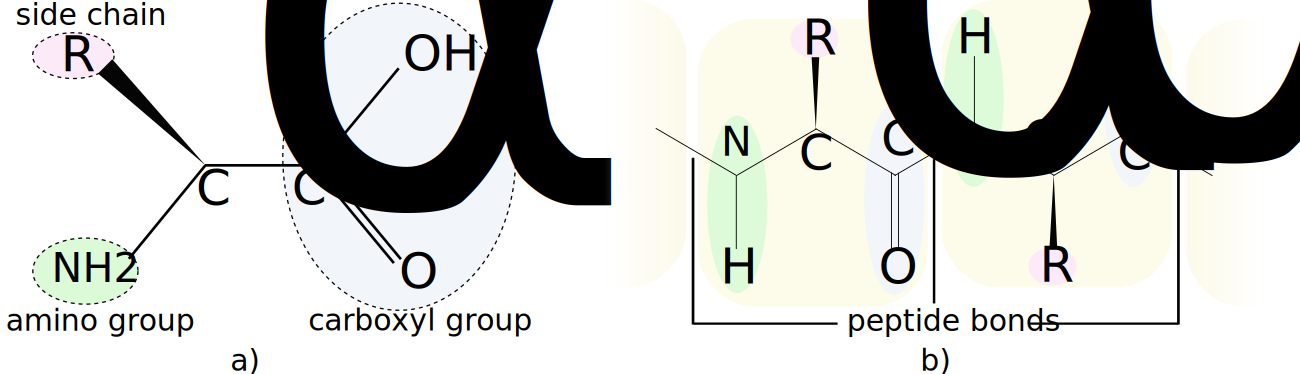
\includegraphics[width=\textwidth]{pictures/aminoacid.pdf} 
  \caption{a) Illustration of a basic amino acid structure. b) Amino acid residues connected into polypeptide chain. It can be noted, that the amino and carboxyl groups are missing atoms, which were released during the formation of peptide bonds as $H_2O$ molecules.}
  \label{Fig:aa}
\end{figure}

During a protein synthesis amino acids are joined together by peptide bonds (covalent bonds), forming polypeptide chains. A peptide bond is formed in a reaction between carboxyl group of one amino acid and amino group of another amino acid (see figure \ref{Fig:aa} b)). As both groups loose atoms that are released as molecule of water during this reaction, the amino acids bonded in polypeptide chains are refereed to as \textit{amino acid residues}. 

Each protein contains at least one long polypeptide chain. This sequence of amino acids, connected by rigid peptide bonds, also known as \textit{backbone}, forms \textit{primary structure} of the protein.

Unlike the peptide bonds, the bonds linking the carboxyl and amino groups to the alpha carbon are free to rotate. Based on these rotations and the patterns of hydrogen bonds that form between hydrogen from amino group and oxygen from corboxyl group, the segments of polypeptide chain can take on various 3D formations. The two most common of those are $\alpha-helices$ and $\beta-sheets$, which are formed by laterally connected $\beta-strands$. These local formations of polypeptide chain are called \textit{secondary protein structures}. Parts of polypeptide chain with absent secondary structures are called \textit{random coils}. See figure \ref{Fig:secondary}.

\begin{figure}[H]
  \centering
  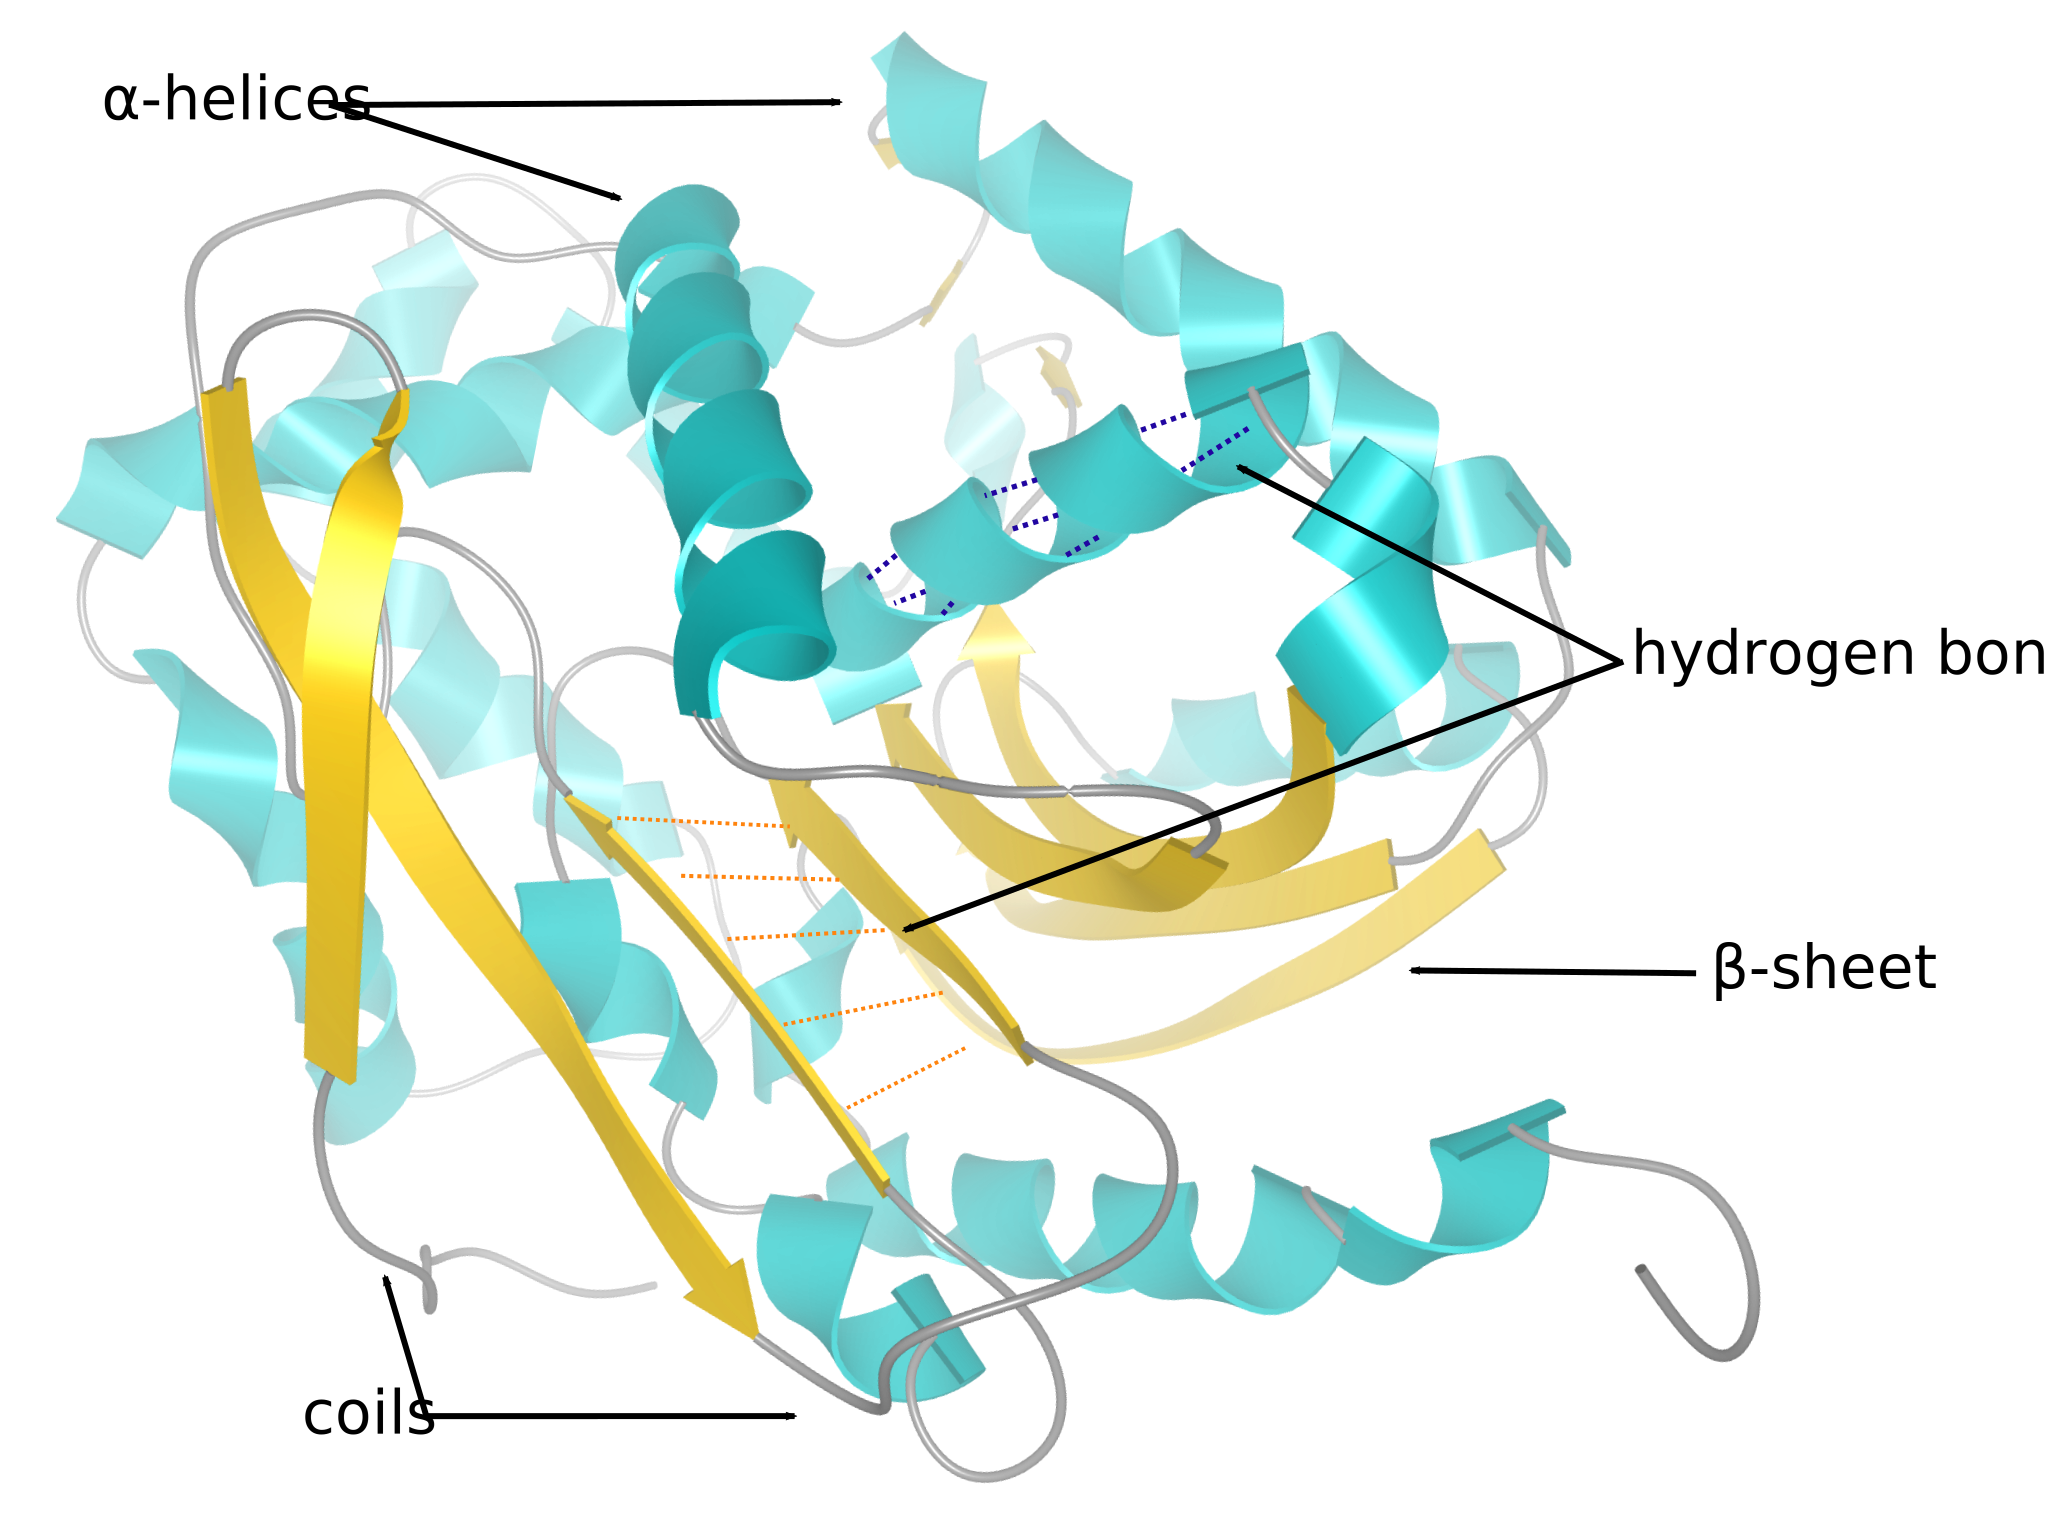
\includegraphics[width=.6\textwidth]{pictures/secondary.pdf} 
  \caption{Typical secondary structures of protein: $\alpha-helices$ (blue), $\beta-strands$ (orange) forming $\beta-sheet$ and \textit{coils}.}
  \label{Fig:secondary}
\end{figure} 

Various side chains of amino acid residues can interact together during the formation of protein. As a result, the secondary structures of the protein are bended and shaped into a  unique 3D structure until the protein attains its minimal energy state. This process is called \textit{protein folding} and it results in a \textit{tertiary protein structure}. The tertiary structure defines the complete spatial arrangement of atoms of one polypeptide chain. Interactions between amino acids of multiple polypeptide chains than define their \textit{quaternary protein structure}.

\subsection{Properties of Proteins}
Previous section described the process of protein attaining its 3D structure. This structure directly influences the way protein is behaving with regards to other molecules and its ability to function properly.

Example of this are the inner voids of the protein. When protein folds, there is naturally some empty space left inside. Depending on the shape of the space we classify four types of inner voids (figure \ref{Fig:voids}): \textit{cavities} -- void space buried deeply inside the protein,  \textit{tunnels} -- connecting cavities with surface of the protein, \textit{channels} -- passing through the whole protein and \textit{pockets} -- shallow dents on the surface of the protein.

\begin{figure}[H]
  \centering
  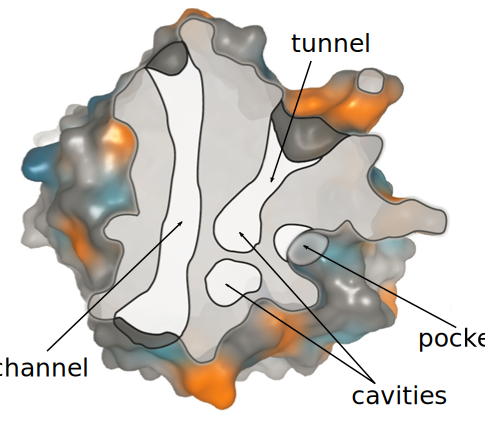
\includegraphics[width=.5\textwidth]{pictures/Voids.pdf} 
  \caption{Types of inner voids of protein. Image adapted from \cite{Strnad2014Thesis}}
  \label{Fig:voids}
\end{figure}

These inner voids can significantly influence the reactivity of the protein since they contain \textit{active site}. Active site is a region of reactive amino acids, where other smaller molecules can bind to protein and undergo a chemical reaction that changes their properties. This place is often buried deep inside the protein and its accessibility is thus limited by the size, shape and physico-chemical properties of the tunnels leading to it. However, the binding site can be located also in shallower pockets on protein surface. In several types of proteins, these binding sites serve for interacting with other proteins.

On the other hand, proteins containing channels (also called pores) occupy entirely different function. They are often found in the membranes of the cells, where the geometry and properties of the channels are responsible for regulating the molecules that can pass through the cell membrane. They are often specific to one type of molecule -- e.g. water, and no other molecules can pass through them in or out of the cell.

As noted above, the reactivity and functions of the proteins are given by their geometry as well as by their physico-chemical properties. These properties are analogous to the properties of the their amino acids:

\begin{itemize}
\setlength\itemsep{0.5pt}
\item{\textit{Polarity and Partial Charge}} \\ 
In a molecule of water, hydrogen atoms are bound to highly electronegative oxygen atom. The electronegativity of oxygen causes higher concentration of electrons on its side of hydrogen bonds and thus a separation of positive and negative electric charge (electric dipole). This phenomenon occurs also in several so called \textit{polar} amino acids. The amount of separated charge is usually lower than fundamental charge, therefore it is called \textit{partial charge}. 
\item{\textit{Donor / Acceptor}} \\
Amino acids participating in hydrogen bonds can be classified as \textit{hydrogen donors} or \textit{hydrogen bond donors} if they contain the hydrogen atoms participating in this bonds. Amino acids on the other side of the bond are called \textit{hydrogen acceptors}. Note that amino acids participating in multiple hydrogen bonds can be donors and acceptors at the same time.
\item{\textit{Hydrophobicity}} \\
 Amino acids are called \textit{hydrophobic} if they seemingly repel water. Unlike \textit{hydrophilic} amino acids, they are not polar and thus cannot create bonds with polar molecules of water.
\end{itemize}

Most of the proteins contain hydrophobic amino acids at their core, while their surface is covered by polar amino acids. They are in contact with outer environment -- \textit{solvent}, where they can form hydrogen bonds.

So far, when discussing the properties of proteins, we have assumed the static 3D structure. However, due to constant physical forces taking place between millions of atoms of proteins and surrounding solvents, the structure of the protein is not static and when studying the proteins one has to consider so called \textit{molecular dynamics (MD)}. This term generally denotes the simulation or the captured interval of atom movement that constantly changes not only the shape but consequently also properties of observed proteins. 

\section{Problem Formulation}
Now that the reader is familiar with basic biochemical terminology, we can formulate the specific problems that will be the focus of this thesis. It was already hinted that proteins can participate in various kinds of intermolecular interactions. In this thesis we will focus on two typical types of interactions: a) protein-ligand interactions and b) protein-protein interactions.

\subsection{Protein-Ligand Interactions} 
In biochemical terminology ligand denotes a small molecule that binds to a protein, where the consequential reaction changes both, the target protein as well as the ligand itself. Analysis of protein-ligand docking (the act of ligand travelling through the protein tunnel and binding to the active site) has application in different fields of biochemistry such as protein engineering or drug design. The typical goal of protein engineering research is changing of protein properties by mutating some of its amino acids to make it, e.g. more stable under high temperature conditions or more reactive with a particular type of ligand. In drug design the goal is to find or adjust protein-ligand combinations, such that their mutual reaction would synthesize new drug from the ligand.
However, in both cases the researchers are looking for the answers to the following questions:
\begin{itemize}
\setlength\itemsep{0.5pt}
\item{Can the ligand pass through the tunnel leading to the active site?}
\item{If not, which parts of the tunnels are causing problems?}
\item{Is it the geometrical bottleneck, that prevents the ligand from passing through the tunnel?}
\item{Are the physico-chemical properties of the tunnel amino acids responsible for repelling the ligand from the active site?}
\item{Can these problems can be resolved by mutating the protein amino acids?}
\end{itemize}

There is already great amount of published work aiming to answer these questions either by studying the tunnel properties or by directly simulating the transportation of the ligand to the active site. However, with the complexity of protein structures in combination with the ever-changing molecular dynamics, the answers are not trivial. Figure \ref{Fig:trajectory} for example depicts trajectory of a ligand in a MD simulation consisting of 50 000 time steps. It is apparent, that further analysis is necessary to identify significant parts and patterns in this simulation. 

\begin{figure}[H]
  \centering
  \includegraphics[width=0.5\linewidth]{pictures/lig_movement.png} 
  \caption{Ligand trajectory (gray) in a simulation containing 50 000 time steps. The protein chain is depicted in blue.}
  \label{Fig:trajectory}  
\end{figure} 

\subsection{Protein-Protein Interactions}
Most of the proteins responsible for various functions in cellular life are operating in larger multi-protein complexes. For example a family of SMC complexes (structural maintenance of chromosomes) govern the organisation of DNA in the cell nucleus. However, in order to interpret their functions properly, it is vital to understand the way the protein are interacting together in these complexes. Mapping the \textit{contact zones} consisting of surface amino acids interacting between the proteins is time consuming process that requires expensive laboratory experiments. Several computational tools therefore aim to reduce the amount of necessary experiments by predicting the possible docking conformations of given proteins. These tools can produce tens to hundreds of possible solutions and it is than up to biochemists to identify the plausible ones. To determine this, the researchers are trying to answer following questions:

\begin{itemize}
\setlength\itemsep{0.5pt}
\item{Which pairs of interacting amino acids are present in a given configuration?}
\item{Which configurations contain a specific interacting pair of
amino acids?}
\item{How close are the amino acids in the contact zone and which
are the closest ones?}
\item{How similar and different are the contact zones in different configurations?}
\item{What are the physico-chemical properties of the amino acids
in the contact zone?}
\end{itemize}

The identification of relevant docking conformations is currently not well supported and the domain experts performing this task by visually comparing the 3D representations of the docked proteins (see figure \ref{Fig:problem}). This approach suffers from high visual complexity, occlusion and imprecise identification of contact pairs of amino acids. It is therefore very difficult to answer the posed questions.

\begin{figure}[H]
  \centering
  \includegraphics[width=0.5\linewidth]{pictures/problem.png} 
  \caption{Superposition of several possible conformations between two proteins. The set of green protein instances corresponds to one of the proteins in the interaction, the colored components represent the second protein in different conformations.}
  \label{Fig:problem}  
\end{figure} 

\subsection{Summary}
In-silico simulations of chemical processes such as molecular docking reduce the time and costs necessary for in-vitro experiments. Yet, the complexity of the generated data almost always calls for further analysis. It is usually up to domain expert to judge the soundness of data and derive conclusions. Without popper tools, this can be difficult and tedious assignment. However, visualization metaphors supporting particular research tasks and  their combinations in an interactive visual analytics's system can significantly speed up the analysis procedure and help with relieving interesting patterns and relationships in data. 

In this work we will present the current state of the art techniques in the visualization and visual analysis of intermolecular interactions of proteins and analyse, how they address the questions posed in the previous sections. We will identify the unsolved problems occurring in the literature, then present the proposed solutions and results that have already been achieved. We will also outline the possibilities for further research.
%%%%%%%%%%%%%%%%%%%%%%%%%%%%%%%%%%%%%%%%%%%
%%%%%%%%%%%%%%%%%%%%%%%%%%%%%%%%%%%%%%%%%%%
%%%%%%%%%%%%%%%%%%%%%%%%%%%%%%%%%%%%%%%%%%%
\chapter{State of the Art}
\label{Sec:star}
In this chapter we will present the state of the art work present in bioinformatical literature with regards to the visualization and analysis of proteins and their interactions with other molecules. We will start with overview of existing molecular visualization techniques, then continue with the work related to protein-ligand interactions, where literature covers a substantial amount of diverse research. The end of this chapter will be dedicated to protein-protein interactions. 

\section{Molecular Visualization}
Many different molecular representations have developed to cater for diverse needs of molecular biologists. Although some new representations are still emerging, the research in this area is currently more focused on development of fast visualization algorithms and GPU-based acceleration of traditional ones, in order to represent large and dynamic molecular data. Here we will provide the overview of typical molecular representations and they state of the art execution. There are, however, countless of other approaches that exceed the capacity of this work. The detailed study concerning molecular representation can be found in state of the art report by Kozlikova et al. \cite{kozlikova2015visualization}. Available is also the report by Patané and Spagnuolo focusing on modeling of molecular surfaces \cite{patane2015state}.

\subsection{Atomistic and Bond-Centric Models}
\begin{wrapfigure}{r}{0.33\textwidth} 
\vspace{-65pt}
  \begin{center}
  \includegraphics[width=0.65\linewidth]{pictures/04_hoffman.jpg} 
  \caption{Hoffman's methane (Marsh-gas) representation \cite{perkins2005history}.}
  \label{Fig:hoffman}  
\end{center}
  \vspace{-30pt}
\end{wrapfigure}

We can say that history of molecular visualization dates back to the 19th century. In 1808 John Dalton published his atomic theory~\cite{dalton1808new}, where he represented atoms and simple molecules with circular shapes. Couple of decades later, around 1860, August Wilhelm von Hoffmann started using first 3D models of molecules in his lectures at Royal Institution of Great Britain~\cite{perkins2005history} -- see Figure \ref{Fig:hoffman}. This type of molecular representation is called \textit{ball-and-stick} model, where balls represent atoms and sticks represent bonds between them. With couple of modifications this representation is commonly used also nowadays (Figure \ref{Fig:vis} b)). 

Over the years other derivations of ball-and-stick model emerged. In 1959 André Dreiding introduced molecular modelling kit using \textit{stick-only} model~\cite{dreiding1959einfache}. Here the atoms were not represented by balls, but merely as connection points between sticks. Nowadays this model is called also \textit{liquorice} or \textit{Dreiding's model} (Figure \ref{Fig:vis} a)). The colouring of the sticks is often used to indicate atoms or their properties.

Although several researchers, including Dalton and Hoffman, claimed that different atoms have different radii, it wasn't until 1873 that the sizes of atoms were experimentally derived by Johannes Diderik van der Waals~\cite{Waals1873PhDThesis}. In later years this discovery led to so called \textit{space-filling} molecular representations, also called \textit{callote} or \textit{CPK models} after chemists Robert Corey, Linus Pauling, and Walter Koltun \cite{corey1953molecular}. In this representation, full "space-filling" sizes of atoms are used, which provides the overview of molecular surface (Figure \ref{Fig:vis} c)).

\begin{figure}[H]
  \centering
  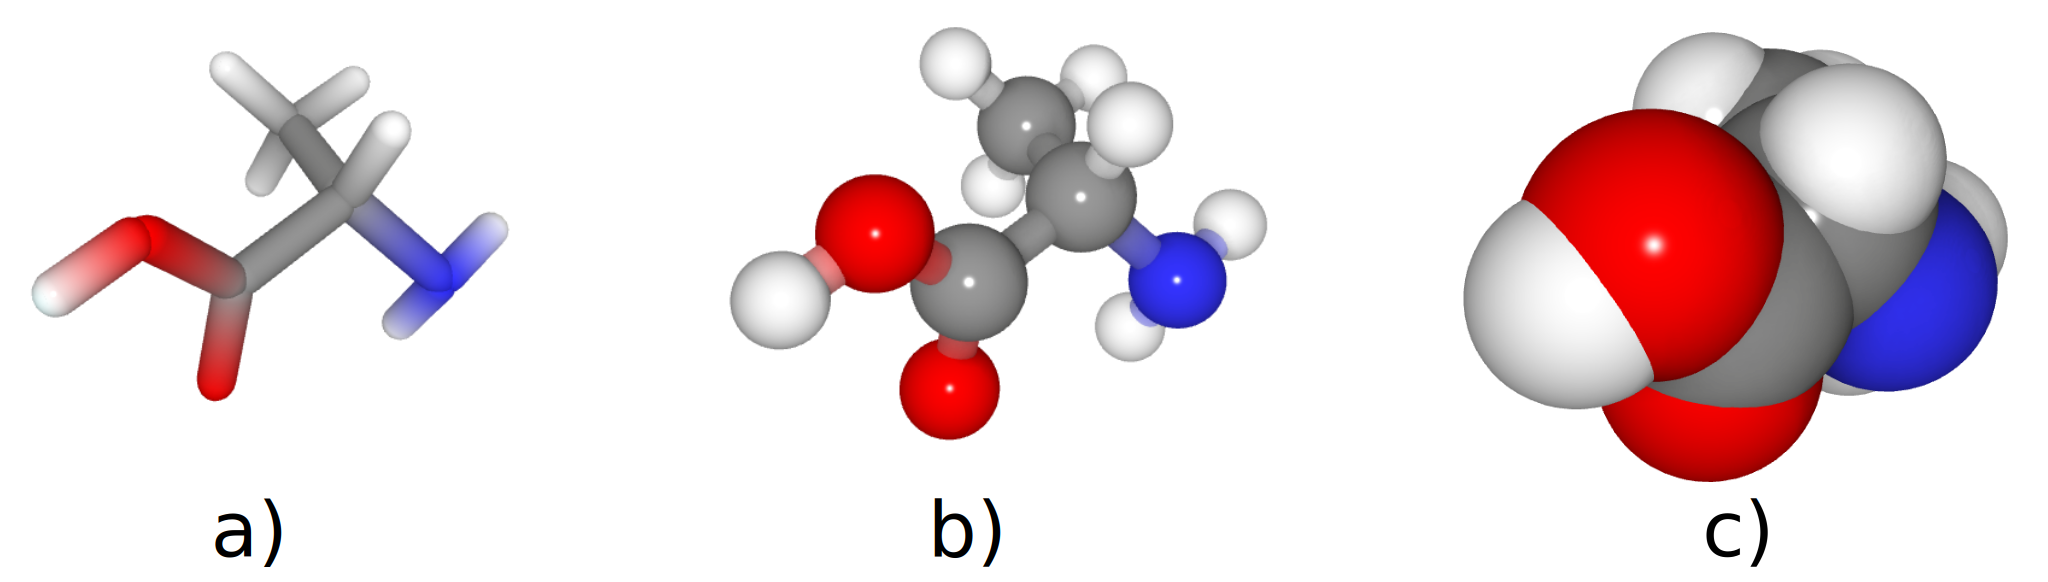
\includegraphics[width=\linewidth]{pictures/vis.pdf} 
  \caption{Types of molecular representations in modern visualization tools: a) liquorice model b) ball-and-stick model c) space-filling model}
  \label{Fig:vis}  
\end{figure} 

Atom and bond based representations of molecules can be decomposed into primitive shapes such as spheres and cylinders, which makes them suitable for GPU-based ray casting. Most of the state of the art rendering techniques stem from glyph ray casting introduce by Gumhold et al. \cite{gumhold2003splatting}, however many performance speedups focusing on rendering of large dynamic molecular structures exist. Since these techniques are focusing on large data samples, they often utilize level of detail (LOD) strategies. Example of this can be the two-level approach of Lampe et al. \cite{lampe2007two} where residues are each residue is represented by one vertex and the atoms in the residues are generated on-the-fly on the GPU. Another approach is used by Le Muzic et al. \cite{le2014illustrative}, where atom positions are stored in a texture and reconstructed using tessellation and geometry shaders.

\subsection{Protein Architecture}
The afore mentioned representations of molecules provide detail information about arrangement of atoms in a molecule. However, for proteins, which can consist of thousands of atoms, this representations can be too cluttered. Therefore, several schematic visualizations were developed.

One of the simplest representations of protein structure is called \textit{alpha trace}. It depicts only the backbone of the protein, as it is derived from the positions of $\alpha$-carbons (Figure \ref{Fig:vis2} a)). This representation provides coarse overview of tertiary and quaternary structure of the protein -- spatial arrangement of the polypeptide chains. However, it can be difficult to identify secondary structures from the alpha trace.

\begin{figure}[H]
  \centering
  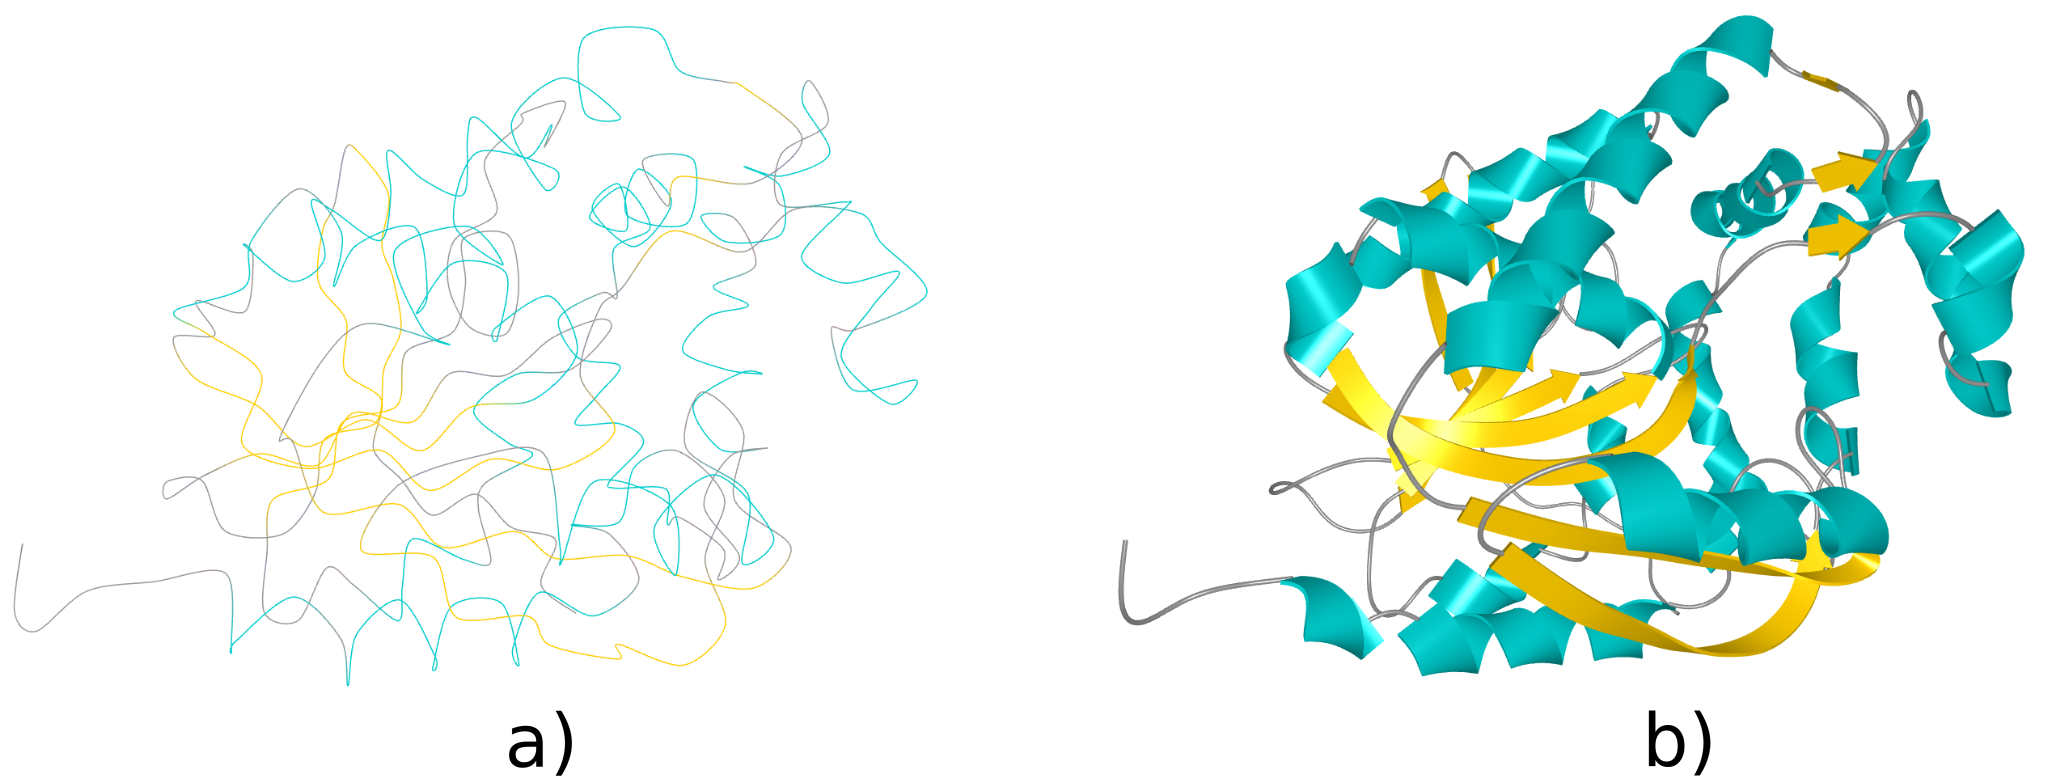
\includegraphics[width=\linewidth]{pictures/representations.pdf} 
  \caption{Types of molecular representations in modern visualization tools: a) alpha trace b) ribbon diagrams}
  \label{Fig:vis2}  
\end{figure} 

In 1981 Jane S. Richardson published \textit{cartoon} illustrations of all then known protein structures \cite{richardson1981anatomy}. In these schematic representations, known today as \textit{ribbon diagrams}, she used consistent and intuitive illustrations of secondary structures to demarcate their position along protein backbone. Although ribbon diagrams were originally hand drawn, they are nowadays part of every molecular visualization software (Figure \ref{Fig:vis2} b)).

Currently the fastes approaches to visualization of ribbon diagrams include the two stage approach by Wahle and Birmanns \cite{wahle2011gpu} where first the backbone tube is generated on CPU and than the vertices are adjusted on GPU to form the final geometry. Another adaptive method by Hermosilla et al. \cite{hermosilla2015instant} takes advantage of the tessellation shader and generates only the geometry needed for current viewpoint.

\subsection{Surface Representations}
\label{Sec:surfaces}
These representations communicate the internal structure of the protein. However in many cases the focus of interest is on the surface of the protein, since the surface is the part of protein that is in contact with outer environment. It is therefore important for biochemists to identify the boundaries of the proteins that are accessible to ligands or interacting with other proteins.

We have already mentioned one type of surface defined by atom spheres of van der Walls radii and therefore called \textit{van der Waals (vdW) surface} \cite{richards1977areas} -- Figure~\ref{Fig:surface} (blue). This surface indicates the precise molecular volume (Figure \ref{Fig:simple} a)).

Another type of surface -- \textit{solvent accesible surface (SAS)} was developed to show the regions of molecule accesible by a solvent molecules \cite{lee1971interpretation}. Here, the solvent molecule is approximated by a spherical probe, which rolls rolls over the vdW surface. The center of the probe than defines the SAS surface -- Figure~\ref{Fig:surface} (yellow). In other words, solvent accesible surface is equal to a vdW surface inflated by the radius of probe.

\begin{wrapfigure}{l}{0.5\textwidth} 
\vspace{-20pt}
\begin{center}
  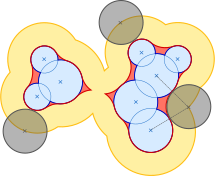
\includegraphics[width=\linewidth]{pictures/surface.pdf} 
  \caption{Schematic representation of molecular surfaces: vdW surface (blue), SES (red) and SAS (yellow). The SES and SAS are defined a probe (grey) rolling over vdW surface. Image taken from \cite{kozlikova2015visualization}.}
  \label{Fig:surface}  
\end{center}
\vspace{-20pt}
\end{wrapfigure}

\textit{Solvent excluded surface (SES)} \cite{richards1977areas} is defined in similar manner to SAS. However, instead of the center of the probe, its outer shell defines the surface -- Figure~\ref{Fig:surface} (red). It was the first smooth surface defined and thanks to the close approximation of molecular volume it is one of the most used surface representations (Figure \ref{Fig:simple} b)). Many algorithms for its computation and visualization have been developed over the years. Currently the fastest soulutions include paralelization of contour-buildap algorithm \cite{totrov1996contour} -- algorithm that computes track of the probe on atom surfaces -- by Lindow et al. \cite{lindow2010accelerated} and Krone et al. \cite{6094043} as well as a grid-based approach by Hermosilla at al. \cite{hermosilla2017interactive} that utilizes progressive surface refinement for rendering of dynamic models on the fly.

\textit{Ligand exluded surface (LES)} is a relatively new generalization of SES proposed by Lindow et al. \cite{lindow2014ligand}. Instead of using an approximate probe, it uses full geometry of ligand to generate the surface. It thus illustrates the precise accessibility, however it is very computationally demanding (Figure \ref{Fig:simple} c)).

Yet another type of molecular surface -- \textit{molecular skin surface (MSS)} was proposed by Edelsbrunner \cite{edelsbrunner1999deformable} (Figure \ref{Fig:simple} c)). The shape of MSS depends on the single parameter \textit{s} -- shrink factor. The advantage of MSS over SES is full $C^1$ continuity.  Among the fastest aproaches to generation of MSS belong the ones by Lindow et al. \cite{lindow2010accelerated} and Yan et al. \cite{Yan2017}.

In 1982 Blinn \cite{blinn1982generalization} proposed use of a Gaussian convolution
kernel to blend atom potentials to achieve an approximation of molecular surface. This technique callled \textit{convolution surface model (CSM)} is more commonly known as Metaballs (Figure \ref{Fig:simple} e)). As with other techniques, improvements and new kernels have been proposed over the years (e.g. by Krone et al. \cite{krone2012fast}) and the resulting techniques belong to the fastest surface rendering approaches. 

\begin{figure}[H]
  \centering
  \includegraphics[width=\linewidth]{pictures/surface2.pdf} 
  \caption{Comparison between different molecular surfaces of the protein isomerase: a) vdW surface b) SES with probe radius 1:4 Å c) LES for equilenine d) MSSwith shrink factor 0.35 e) Gaussian surface with standard deviation equal to the atom radius. Image taken from \cite{kozlikova2015visualization}.}
  \label{Fig:surface2}  
\end{figure}

\subsubsection{Surface Simplification}
With larger kernels, the CMS can be used for simplification of molecular surface, showing just the general shape of the protein. This is sometimes required, as molecular surfaces are often used for mapping of other properties of proteins and atomistic models with many occlusions and high visual complexity are not suitable for this purpose.

Couple of other approaches for surface simplification have been proposed. \textit{Coarse graining} \cite{levitt1976simplified} is method that groups several atoms (e.g. one amino acids) together. These groups are than represented by single sphere. Another approach is mapping the molecular surface to spherical coordinates \cite{postarnakevich2009global}.

\begin{wrapfigure}{l}{0.5\textwidth} 
\vspace{-10pt}
  \begin{center}
  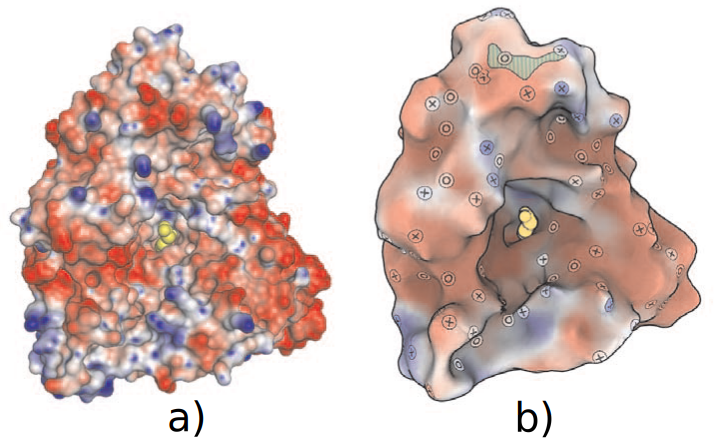
\includegraphics[width=0.95\linewidth]{pictures/simpl.pdf} 
  \caption{Simplified surface representation proposed by Cipriano and Gleicher. a) SES b) simplified surface. Image taken from \cite{cipriano2007molecular}.}
  \label{Fig:simple}  
	\end{center}
  \vspace{-30pt}
\end{wrapfigure}

Cipriano and Gleicher \cite{cipriano2007molecular} proposed a method that uses a combination of
filters and mesh restructuring to smooth the low frequency parts of the surface and generate a simplified representation of overall shape of the protein (see Figure \ref{Fig:simple}). Markings are then placed on the surface to indicate the important removed details as well as other features of the surface, such as the physico-chemical properties of surface amino acids.

\subsubsection{Visual Enhancements}
Another way of dealing with high visual complexity of molecular structures is introduction various visual enhancements. One the most employed visual cues in molecular rendering is certainly \textit{ambient occlusion (AO)} \cite{miller1994efficient}. The goal of this technique is to calculate, how each object in the scene is exposed to the ambient lighting. It is computationaly very expensive, however the latest results from Hermosilla et al. \cite{hermosilla2016high} enable real time rendering of AO for MD simulations.

In their work, they also cover rendering of another common effect -- \textit{halos}. Haloes are highlights extending from selected object boundaries (used e.g. to indicate ligand in an MD simulation). Similar to them are also \textit{depth-dependent silhouettes}, that contour the edges  detected from scene depth map. Another effect for guidance of attention was adapted from photography -- \textit{Depth of Field} simulation blurs the objects that are out of focus. 
Other rendering techniques, such as \textit{toon shading}, \textit{line drawing} and \textit{hatching} are commonly used for molecular rendering as well, since they can be adjusted to emphasize important features \cite{kozlikova2015visualization}.

%\subsection{Molecular Visualization Systems}

\section{Analysis of Protein Voids}
We have described many possible representations that support the analysis of proteins in general. In this section, we will focus on one of the most important features of proteins -- their inner voids. As we mentioned before, the active site -- the reactive area of the protein is often buried deeply inside of the protein structure and accessible only via those voids, namely tunnels. Therefore, the extraction and analysis of these tunnels is vital for the study of protein-ligand binding. Here, we will mention only several most videly used principles of the approaches used in this area, as the extensiveness of this work exceeds the capacity of this thesis. Complete overview of the published tools for detection and analysis of biomolecular cavities can be found in state of the art reports by Krone et al. \cite{krone2016visual} and Simões et al. \cite{simoesgeometric}.

\subsection{Detection of Protein Voids}
There are several methods for extracting the shape of the protein voids in general, as well as numerous ones focusing on tunnels specifically. The algorithms can be classified into several categories, depending on the approach they use: grid-based, probe-based, Voronoi-based, surface-based, path analysis and ligand based. Most of the algorithms combine several approaches, in order to achieve better results. Moreover, we can differentiate  between algorithms applicable only for static structures and algorithms taking into account molecular dynamics.

Many algorithms for void detection use a voxel grid to subdivide the 3D space containing the protein. The basic ide of purely \textit{grid-based approaches} is to split voxels into two groups -- those that lie inside a protein atoms and those that lie in a void space. 
The grid points from the second group are then assigned value based on different properties -- distance to the protein atoms (\cite{levitt1992pocket, Petrek2006Caver, hendlich1997ligsite}), interaction energies (\cite{an2005pocketome, laurie2005q, hernandez2009sitehound}) or protein and solvent 
\begin{wrapfigure}{r}{0.5\textwidth}
\vspace{-17pt}
  \begin{center}
  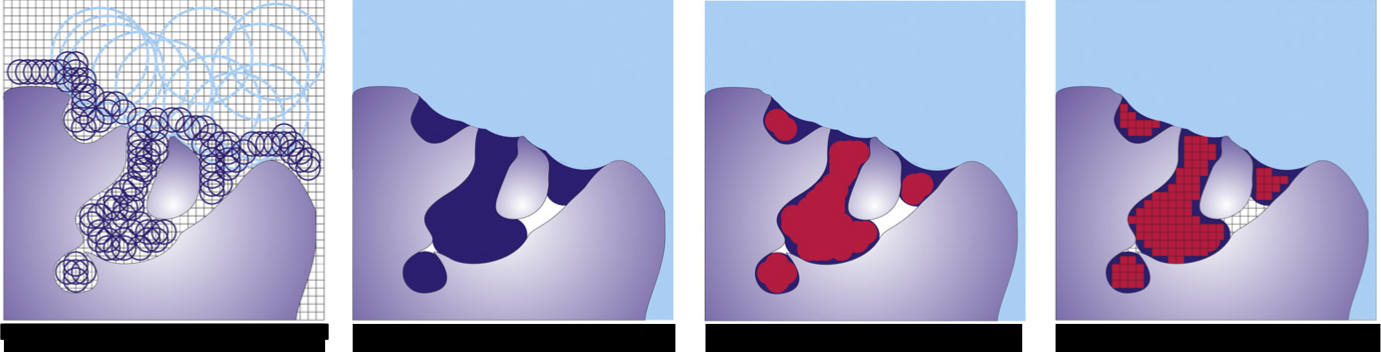
\includegraphics[width=\linewidth]{pictures/rollingprobe.pdf} 
  \caption{Rolling probe method. a) Two kinds of probes are placed in each point of the grid. b) The identified volumes are divided into the protein surrounding (light blue), and internal voids (red). Dark blue areas indicate undetected internal volume. Image adapted from \cite{brezovsky2013software}.}
  \label{Fig:rollingprobe}  
	\end{center}
  \vspace{-25pt}
\end{wrapfigure}
residence probability extracted from MD simulation (\cite{raunest2011dxtuber, krone2011interactive, kokh2013trapp, paramo2014efficient}). The evaluated grid is further processed to extract the cavities using e.g. flood-fill segmentation or path analysis to find the cheapest path from active site to the surface of the protein.
%An exaple of a \textit{grid-based approach} that also utilizes \textit{path analysis} is the first version of CAVER algorithm \cite{Petrek2006Caver}. Here, each node of the grid is assigned a cost, based on the maximal radius of a hypothetical ball that can be inserted into a node without intersecting voxels occupied by protein atoms -- the larger the radius, the lower the cost. A graph searching algorithm than searches for cheapest path leading from user defined active site to the outer boundary of protein. This path is than taken as tunnel centreline and the detected tunnel is tan represented as a set of maximal spheres placed on centreline.

Second group of algorithms utilizes \textit{grid-based approaches} in combination with  \textit{probe-based approaches}. For example, HOLLOW \cite{Ho2008Hollow} and 3V \cite{voss20103v} algorithms use two probe spheres of different sizes that are placed in each node of the grid (see Figure \ref{Fig:rollingprobe}). The probes that do not intersect with protein atoms define the surface of the protein -- large probe defines the outer surface, while the smaller one defines also the inner voids. This approach is also referred to as \textit{rolling probe} principle. Different combinations probe-based and grid-based approaches can be found e.g. in \cite{kleywegt1994detection, czirjak2015princces, laskowski1995surfnet, yu2009roll}.

\begin{wrapfigure}{l}{0.6\textwidth}
\vspace{-17pt}
   \begin{center}
  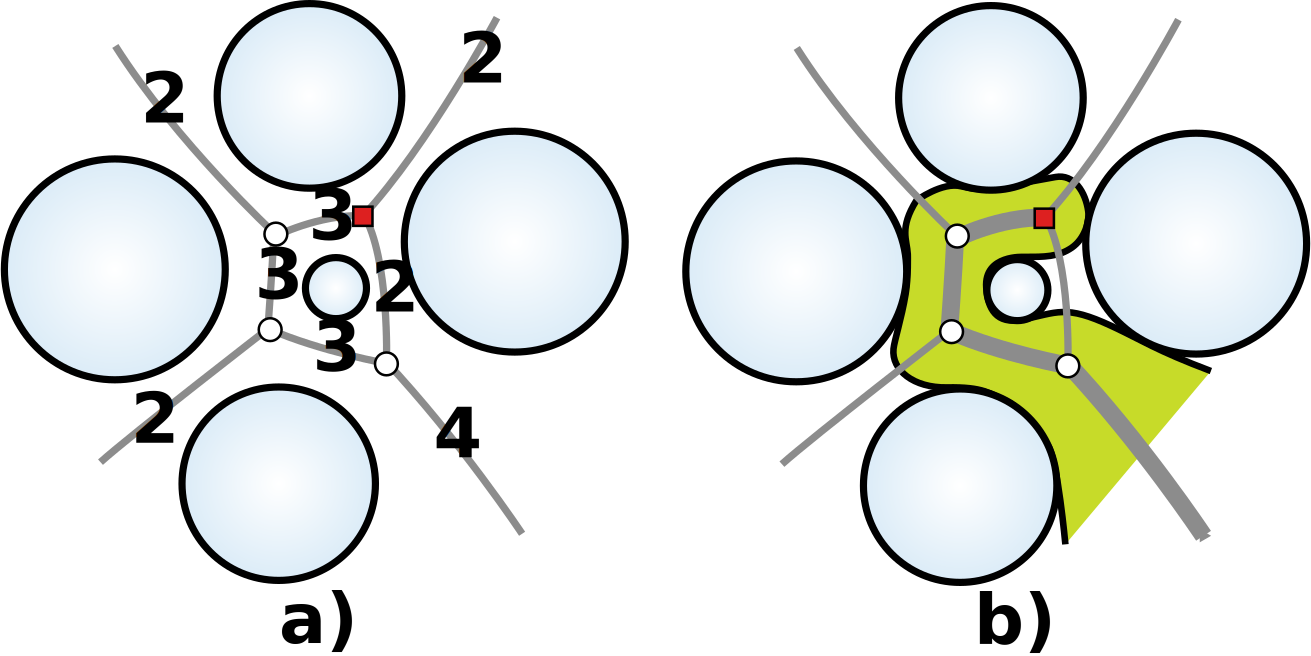
\includegraphics[width=\linewidth]{pictures/voronoi.pdf} 
  \caption{Example of Voronoi-based tunnel detection. a) Evaluated edges. b) Path with highest score found by Dijkstra's algorithm. Red square indicates active site. Image adapted from~ \cite{caver20}}
  \label{Fig:voronoi} 
   \end{center} 
   \vspace{-17pt}
\end{wrapfigure} 

Accuracy of grid-based algorithms strongly depends on the resolution of the voxel grid. At the same time, high resolution of the grid leads to high memory demands of these algorithms. \textit{Voronoi-based} algorithms in combination with \textit{path analysis} address these drawbacks by utilizing Voronoi diagrams to subdivide the 3D space of protein structure (see Figure \ref{Fig:voronoi}). Each atom of the protein forms a center of Voronoi cell. The edges are then evaluated by cost function, which assigns the value based on distance of the edge from the cell centres (i.e. atom centres). Then, Dijkstra's algorithm is used on the edge graph to find the best path from the active site towards protein surface. This principle is used and improved upon in \cite{Petrek2007MOLE, caver20, Yaffe2008MolAxis}. Chovancova et al.~\cite{caver30} extend this approach for detection of tunnels taking into account the movement of the protein in CAVER 3.0 algorithm. It computes tunnel paths for each time frame of MD simulation. Than the corresponding paths are clustered. Thus it is possible to track the evolution of the tunnels in time.

Another set of void detection methods is based on theory of $\alpha$-shapes. First, they compute Voronoi diagram on the atoms of the protein in a same manner as previous methods and transform it to Delaunay triangulation. Than, all the triangles that do not lie completely inside the protein atoms are deleted, resulting in an $\alpha$-shape of the protein. The cavities can than be easily extracted from the $\alpha$-shape. This method was first used in CAST~\cite{liang1998anatomy} and was later extended and generalized by \cite{sridharamurthy2016extraction, kim2013tunnels, masood2015chexvis}.

In 2011 two new approaches \cite{olechnovivc2010voroprot, Lindow2011Voronoi} appeared using weighted \textit{Voronoi diagrams} of atom spheres in combination with \textit{probes}. For each Voronoi vertex of these diagrams an empty sphere tangent to four atom spheres exists. If the sphere is larger than a size of probe it is consider to be a cavity. Since this approach considers the atom radii, it produces geometrically optimal results for probe spheres.

In Section \ref{Sec:surfaces} we have described several methods for extraction of molecular surfaces. Based on these methods, several \textit{surface-based} approaches for detection of cavities have been proposed. For example, Jurčík et al. \cite{jurvcik2016accelerated} extend the method proposed for computation of SES by Krone et al.~\cite{6094043} to detect also closed cavities. Coleman and Sharp \cite{Coleman2009CHUNNEL} use triangulation of SES to detect channels in proteins. Krone et al. \cite{krone2013interactive} proposed a method for real time GPU accelerated extraction of cavities based on Ambient Occlusion. The LES method proposed by Lindow et al. \cite{lindow2014ligand} enables extraction of cavities based on the actual geometry of the ligand.

The tunnel detection can be alternatively viewed as a path planning problem -- the task is to find a collision free path for ligand starting at active site and leading to the surface. Path planning approaches to tunnel detection usually employ Rapidly Exploring Random Trees \cite{lavalle1998rapidly} (RRT), a technique that builds a tree of collision free configurations moving through the defined space. This approach can be applied directly on an MD simulation, thus it avoids the computationally expensive step of traditional, e.g. Voronoi-based approaches, where correspondence between geometry computed in different MD snapshots has to be found. Most notable work in this are includes \cite{cortes2005path, vonasek2016application, vonasek2017tunnel}.

\subsection{Visual Analysis of Protein Tunnels}
Spatial visual representations of molecular tunnels correspond to traditional molecular visualizations. The most simple tunnel representation consist of set of spheres placed along the tunnel centreline -- the radius of each sphere corresponds to the maximal probe that fits into the tunnel at given place without intersecting with molecular atoms. Optionally tunnel centreline can be displayed as well. 

We have already mentioned several surface-based methods for cavity detection that consequently use surface visualization to depict the detected cavities. Those methods also propose visual enhancements to highlight the cavities within the context of molecule -- e.g. customized clipping planes, modulated coloring \cite{parulek2012implicit} or transparency of molecular srface \cite{jurvcik2016accelerated} or selective lighting \cite{Lindow2011Voronoi}. 

Moreover, several systems interactively combine 3D view and abstracted 2D plots to support the analysis of detected tunnels. Lindow et al. \cite{Lindow2012DynamicChannels, Lindow2013DynamicCavities} proposed an interactive tool for analysis of changes in the cavities in molecular dynamics. The tool includes interactive relational graph, that plots the evolution of the position and size of the cavities, as well as their splits and merges. On demand it offers 3D overview of aggregated shaped of selected cavity traced through the MD simulation. Similar principles were also utilized by Krone et al. {krone2014visual}.

Byška et al. \cite{byvska2016animoaminominer} presented a tool that combines line plot showing the tunnel width profile with a list of amino acids that influence the tunnel at different time steps of an MD simulation. By interaction it is possible to find the amino acids that might cause tunnel bottlenecks. Byška et al. \cite{byvska2015molecollar} also presented another tool for exploration of evolution of molecular tunnel. In this work they employed filterable heat maps to provide width overview for multiple detected tunnels as well as more detailed view based on tunnel cross-cuts which again plots surrounding amino acids. 

Yet another approach to tunnel analysis was presented by Kolesár er al.~\cite{kolesar2016unfolding}. This work presents a method for comparison and analysis of tunnels based on unfolding of a 3D surface and flattening it into 2D map-like representation that denotes the amino acids surrounding the tunnel. These 2D representations can than be clustered and compared using image processing methods. 

\begin{figure}[t]
  \centering
  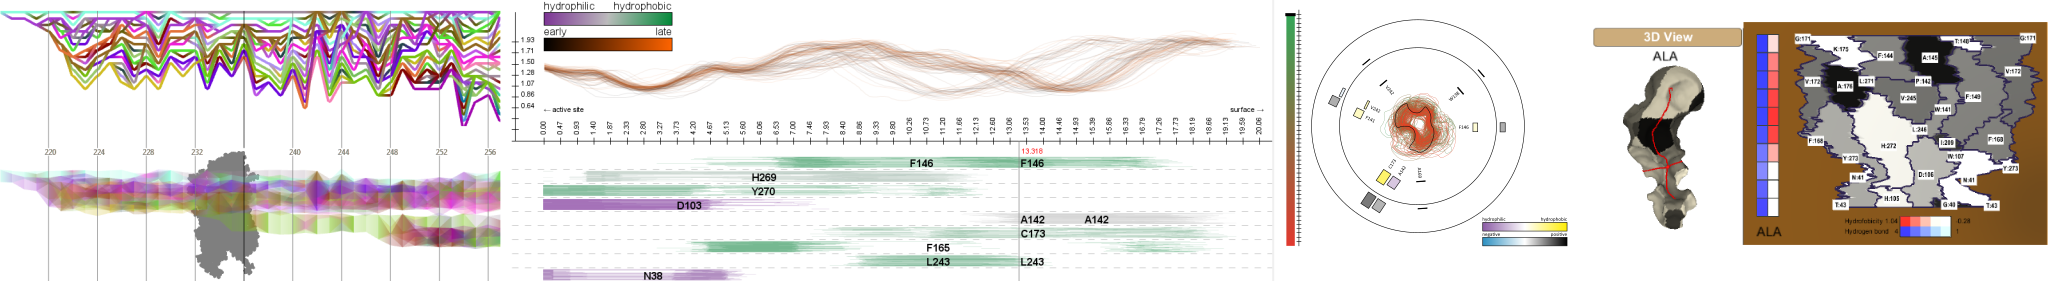
\includegraphics[width=\linewidth]{pictures/tunnels.pdf} 
  \caption{a) Relational graph by Lindow et al. \cite{Lindow2013DynamicCavities} b) AnimoAminoMiner\cite{byvska2016animoaminominer} c)MoleCollar \cite{byvska2015molecollar}, d) Tunnel unfolding by Koles8r et al. \cite{kolesar2016unfolding}.}
  \label{Fig:tunnels}  
\end{figure}


%ligand md simulations

\section{Protein-Protein Interactions}

\subsection{Docking}
\subsection{Visual Analysis}

%%%%%%%%%%%%%%%%%%%%%%%%%%%%%%%%%%%%%%%%%%%
%%%%%%%%%%%%%%%%%%%%%%%%%%%%%%%%%%%%%%%%%%%
%%%%%%%%%%%%%%%%%%%%%%%%%%%%%%%%%%%%%%%%%%%
\chapter{Aims of the Thesis}
\label{Sec:Aims}
\section{Protein-Ligand Interactions}
-flexible ligand
\section{Protein-Protein Interactions}
-visualization of multi-protein complexes
-visual analysis of (template)docking of homology-modelled proteins
\section{Study Plan}
\begin{itemize}
\renewcommand{\labelitemii}{$\circ$}
\item{Autumn 2017}
		\subitem{Autumn 2017}
\item{Spring 2018}
\item{Autumn 2018}
\item{Spring 2019}
\item{Autumn 2018}
\end{itemize}
%CAPRI evaluation
%homology 
%%%%%%%%%%%%%%%%%%%%%%%%%%%%%%%%%%%%%%%%%%%
%%%%%%%%%%%%%%%%%%%%%%%%%%%%%%%%%%%%%%%%%%%
%%%%%%%%%%%%%%%%%%%%%%%%%%%%%%%%%%%%%%%%%%%
\chapter{Achieved Results}
\label{Sec:Results}



%%%%%%%%%%%%%%%%%%%%%%%%%%%%%%%%%%%%%%%%%%%
%%%%%%%%%%%%%%%%%%%%%%%%%%%%%%%%%%%%%%%%%%%
%%%%%%%%%%%%%%%%%%%%%%%%%%%%%%%%%%%%%%%%%%%
%%%%%%%%%%%%%%%%%%%%%%%%%%%%%%%%%%%%%%%%%%%
%%%%%%%%%%%%%%%%%%%%%%%%%%%%%%%%%%%%%%%%%%%
\renewcommand{\thesection}{\arabic{section}}
%%%%%%%%%%%%%%%%%%%%%%%%%%%%%%%%%%%%%%%%%%%
%%%%%%%%%%%%%%%%%%%%%%%%%%%%%%%%%%%%%%%%%%%
%%%%%%%%%%%%%%%%%%%%%%%%%%%%%%%%%%%%%%%%%%%
\chapter{Author's Publications}
\label{Sec:Publications}

%\printbibliography[title=References]
\bibliography{thesis}{}
\bibliographystyle{plain}        


\end{document}